\documentclass[addpoints,12pt]{exam}

\usepackage[margin=.75in,tmargin=.9in,bmargin=1in,letterpaper]{geometry}
\usepackage{tikz}
\usepackage{siunitx}
\usepackage{lastpage}
\usepackage{newtxtext,newtxmath}

\usetikzlibrary{decorations.pathmorphing,patterns}

\setlength{\parindent}{0pt}
\setlength{\parskip}{0pt}

\sisetup{
  inter-unit-product =\cdot,
  per-mode=symbol,
}
\tikzset{
  >=latex
}
\renewcommand{\choiceshook}{
  \setlength{\leftmargin}{22pt}
  \setlength{\itemsep}{0pt}%.9\baselineskip}
  \setlength{\topsep}{0pt}
  %\setlength\partopsep{100pt} 
  \setlength\parsep{0pt}
}


\pagestyle{headandfoot}
\header{Meritus Academy}{}
       {Physics 12 Midterm Test (Page \thepage/\pageref{LastPage})}
\footer{}{}{}

%\pointsinmargin
\bracketedpoints
\pointpoints{mark}{marks}
\bonuspointpoints{bonus mark}{bonus marks}
%\setlength\answerskip{0ex}
%\setlength\answerlinelength{.5in}
%\hpword{Marks:}

\begin{document}

\vspace{.6in}
\makebox[\textwidth]{
  Student Name: \underline{\hspace{2.2in}}\hspace{.3in}
  Teacher Name: \enspace\hrulefill
}

\begin{center}
  \vspace{.2in}
  {\Large\textbf{Grade 12 Physics (Take Home) Midterm Test}}
  \vspace{.15in}
  
  \fbox{\parbox{7in}{
      \textbf{Instructions:}
      This midterm test has nineteen questions: 8 multiple-choice questions,
      %3 short-answer questions,
      6 problem-solving questions, and 1 bonus
      question. For problem-solving questions, all work \emph{must} be shown.
      Correct answers without full solution will not receive a passing mark.
      Each question is assigned different mark values. The bonus question is
      worth 10 marks. The maximum mark that you can get is 110 out of 100.
      Please put a box around all your answers. Answer all questions to
      \textbf{three significant figures}. Answer the questions in the space
      provided.%; attached additional work on separate sheets of paper if more
      %space is required.
    }
  }

%  \vspace{.25in}
%  \gradetable[h][questions]
%  \vspace{.15in}
\end{center}

\textbf{Multiple-Choice Questions:} Read each question carefully and select
the \emph{best} response for each question.

\vspace{.1in}For \emph{online} classes: answer all questions using the
Classkick app by clicking on the selection box on the right of each question.
Do \emph{not} use the pen function, and do \emph{not} upload image files for
this section. Marks will only be awarded if instructions are followed.

\vspace{.1in}For \emph{in-person} classes: please answer all question by
writing your answer in the space on the right.

\vspace{.1in}Part marks \emph{may} be awarded if work is shown.

\begin{questions}
  \question[2] Comparing an object that is \emph{dropped}, and an identical
  object \emph{thrown horizontally} from the same height at the same time, the
  time it takes to hit the ground \underline{\hspace{1in}}
  \begin{choices}
    \choice is less for the thrown object
    \choice is the same for each object
    \choice is greater for the thrown object
    \choice depends on the initial velocity of each object
    \choice cannot be calculated without additional information
  \end{choices}
  \vspace{-.2in}\answerline
  
  \question[2] A car travels with a constant speed around a curve in the road.
  The curve is banked at an angle $\theta$. Which of the following forces is in
  the direction of the net force on the car?
  \begin{choices}
    \choice The horizontal component of the force of gravity
    \choice The static friction force
    \choice The horizontal component of the normal force
    \choice The force of gravity
    \choice The centrifugal force
  \end{choices}
  \vspace{-.2in}\answerline
    
  \question[2] When an object is in uniform circular motion, the direction of
  the acceleration is \underline{\hspace{.5in}}
  \begin{choices}
    \choice directed tangent to the circle
    \choice directed towards the centre of the circle
    \choice changing depending on its position in the circle
    \choice directed outward from the centre of the circle
    \choice opposite to the direction of centripetal force
  \end{choices}
  \vspace{-.25in}\answerline
  \newpage
  
  \question[2] If the mass of a car is double and its speed is tripled, then
  the kinetic energy changes by a factor of \underline{\hspace{.6in}}
  \begin{choices}
    \choice 0.67
    \choice 6
    \choice 1.5
    \choice 18
    \choice 6
  \end{choices}
  \vspace{-.2in}\answerline
    
  \question[2] To catch a water-filled balloon without breaking it, people
  allow their hands to move with the balloon upon catching it. This works
  because \underline{\hspace{1in}}
  \begin{choices}
    \choice the balloon's momentum changes more slowly
    \choice there is less force applied
    \choice there is less impulse
    \choice two of A, B, and C
    \choice all of A, B, and C
  \end{choices}
  \vspace{-.2in}\answerline
    
  \question[2] You throw a rock straight up into the air. While it rises and
  falls, its kinetic energy \underline{\hspace{.6in}}
  \begin{choices}
    \choice remains constant
    \choice increases steadily
    \choice changes direction only
    \choice decreases then increases
    \choice increases then decreases
  \end{choices}
  \vspace{-.2in}\answerline
  
  \question[2] A satellite orbits Earth at a constant speed. Which of the
  following statements are true?
  \begin{choices}
    \choice There is a force on the satellite towards the centre of the orbit.
    \choice There is a force on the satellite pulling it out away from the
    centre of the orbit.
    \choice There is a force on the satellite along the direction of its motion.
    \choice There are forces both along the direction of motion and towards
    the centre.
    %\choice Jupiter is accelerating towards the centre of the orbit.
    \choice There are no forces on the satellite.
  \end{choices}
  \vspace{-.2in}\answerline
    
  \question[2] Two satellites orbit Earth at the same speed in identical
  orbits. Satellite A is twice the mass of Satellite B. How does the centripetal
  acceleration of Satellite A compare with that of Satellite B?
  \begin{choices}
    \choice Four times as much
    \choice Twice as much
    \choice The same
    \choice One-half as much
    \choice One-fourth as much
  \end{choices}
  \vspace{-.2in}\answerline
  \newpage
    
%  \question[2] Which of the following is defined as ``the rate of change of
%  velocity''?
%  \begin{choices}
%    \choice Distance
%    \choice Displacement
%    \choice Acceleration
%    \choice Jerk
%    \choice Speed
%  \end{choices}
%  %\vspace{-.2in}\answerline
%    
%  \question[2] Which of the following is defined as ``the change in position of
%  an object relative to a reference point''?
%  \begin{choices}
%    \choice Distance
%    \choice Displacement
%    \choice Velocity
%    \choice Acceleration
%  \end{choices}
%  %\vspace{-.2in}\answerline
%  %\end{parts}

% THIS QUESTION IS REMOVED FOR THE WINTER 2019 MIDTERM. IT'S NOT A BAD
% QUESTION, AND MAY BE ADDED AGAIN IN A LATER TIME.
%\question[8] A \SI{485}{\kilo\gram} elevator is rated to hold 15 people of
%  average mass (\SI{65}{\kilo\gram}). The elevator cable can withstand a maximum
%  tension of \SI{3.74e4}\newton, which is twice the actual maximum force that
%  the load will create (\SI{200}{\percent} safety factor). What is the greatest
%  upwards acceleration that the elevator
%  can have with the maximum load? (Hint: start with a free-body diagram.)
%\vspace{2in}

  \fullwidth{
    \textbf{Short-Answer Questions:} %Please answer all the questions using the
    %text box directly on Classkick. There are no calculations for this section.
  }
  \question[5] A rubber ball is dropped, bouncing on the floor. Would the
  collision between the ball and the floor be elastic or inelastic? What
  physical observations would lead to this conclusion?
  \vspace{\stretch1}

  \question[5] Is it possible that the net (i.e.\ total) kinetic energy for two
  objects be non-zero while the net momentum is zero? Explain, or give an
  example.
  \vspace{\stretch1}
  \newpage
  
%  \question[4] A crate rests on a ramp with an angle of inclination $\theta$
%  without sliding. As one end of the ramp is raised further, the angle $\theta$
%  increases, causing the crate to start slide. Explain why this happens. (There
%  are two reasons. Hint: what happens to each individual forces acting on the
%  ramp.)
%  
%  \begin{tikzpicture}[scale=2]
%    \begin{scope}[thick]
%      \begin{scope}[rotate=30]
%        \draw(0,0)--(2,0);
%        \draw(1,0) rectangle(1.75,.5);
%      \end{scope}
%      \draw[->](.75,0) arc(0:30:.75) node[pos=.6,right]{$\theta$};
%      \draw(0,0)--(2,0);
%    \end{scope}
%  \end{tikzpicture}
%  \vspace{1in}
%  \newpage


  \fullwidth{
    \textbf{Problem-Solving Questions:} Please do all your work on a separate
    piece of paper, and upload to the test as a clear \emph{black-and-white}
    image. Alternatively you may also obtain the PDF file from your teacher,
    and do your work electronically using an annotator software.
  }

  \question A cannon located atop the edge of a \SI{234.5}{\metre} cliff fires
  a cannonball that hits an enemy target \SI{4.65}{\kilo\metre} away from the
  base of the cliff. If the cannonball is launched at an angle of \ang{36.9}
  above the horizontal. If air resistance can be ignored,
  \begin{parts}
    \part[6] What is the initial speed $\varv_0$ of the cannonball?
    \part[6] How long does it take ($\Delta t$) to hit the enemy target?
  \end{parts}
  (Hint: Write down the kinematics equation for both horizontal and vertical
  directions. There will be two variables that you will need to solve, and two
  equations to solve them. It does not matter which part of the question you
  solve first.)
  \newpage

%  \question A \SI{2.0}{\kilo\gram} block sits on a \SI{4.0}{\kilo\gram} block
%  that is resting on a table, as shown below. The coefficients of static and
%  kinetic friction between the blocks are $\mu_s=0.30$ and $\mu_k=0.20$,
%  respectively. There is no friction between the \SI{4.0}{\kilo\gram} block and
%  the table.
%  \begin{center}
%    \begin{tikzpicture}[scale=1.4]
%      \begin{scope}[thick]
%        \draw (-1,0)--(4,0);
%        \draw[fill=gray!70] rectangle(2,1) node[midway]{\SI{4.0}{\kg}};
%        \draw[fill=gray!40](.5,1)rectangle(1.5,1.75)node[midway]{\SI{2.0}{\kg}};
%      \end{scope}
%      \draw[ultra thick,->](2,.5)--(3.5,.5) node[right]{$\vec F$};
%    \end{tikzpicture}
%  \end{center}
%  \begin{parts}
%    \part Draw
%    
%    \part What is the maximum force $\vec F$ that can be applied if the
%    \SI{2.0}{\kilo\gram} block is not to slide on the \SI{4.0}{\kilo\gram}
%    block.
%    \label{partA}
%    
%    \part If $\vec F$ is half this value, find the acceleration of each block
%    and the force of friction acting on each block.
%    
%    \part If $\vec F$ is twice the value found in (\ref{partA}), find the
%    acceleration of each block.
%  \end{parts}
%  \newpage

  \question A \SI{450}{\gram} wooden block ($A$) on a horizontal table top is
  connected to a suspended \SI{150}{\gram} mass ($B$) by a string passing over a
  frictionless pulley. The coefficient of friction between $A$ and the table is
  0.08.
  \begin{center}
    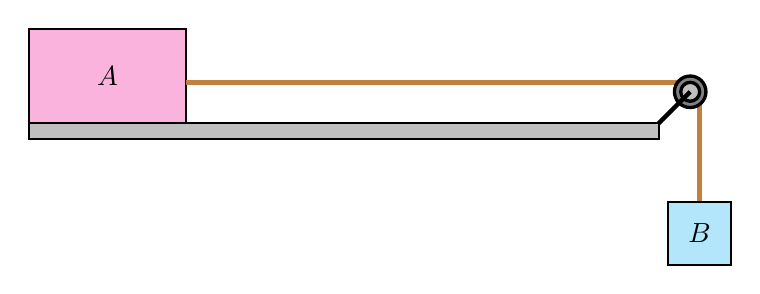
\begin{tikzpicture}[scale=2]
      \begin{scope}[thick]
        \draw[fill=lightgray] rectangle (4,-.1);
        \draw[fill=magenta!30] rectangle (1,.6) node[midway]{$A$};
        \draw[ultra thick, brown] (1,.26)--(4.2,.26);
        \draw[ultra thick, brown] (4.26,.2)--(4.26,-.5);
        \draw[very thick,fill=gray] (4.2,.2) circle (.1);
        \draw[very thick,fill=lightgray] (4.2,.2) circle (.06);
        \draw[ultra thick] (4,0)--(4.2,.2);        
        \draw[fill=cyan!30] (4.06,-.5) rectangle (4.46,-.9) node[midway]{$B$};
      \end{scope}
    \end{tikzpicture}
  \end{center}
  \begin{parts}
    \part[4] Draw free-body diagrams of the blocks at the moment they are
    released.
    \part[4] Calculate the acceleration of the blocks.
    %\part[2] How long will it take Block A to travel \SI{1.1}\metre?
    \part[4] Calculate the tension of the string while the blocks are
    accelerating.
  \end{parts}
  \newpage
  
  \question You are a passenger on an airplane and you decide to measure its
  acceleration as it speeds up along the runway during take-off. Your take out
  a yo-yo and notice that when you suspend it, it makes an angle of
  \ang{35} with the vertical. The airplane's take-off mass is
  \SI{2.54e5}{\kilo\gram}.
  \begin{parts}
    \part[3] Draw a free-body diagram of the yo-yo.
    \part[3] Determine the acceleration of the airplane.
    \part[3] If the yo-yo's mass is \SI{65}\gram, what is the tension in the
    string?
  \end{parts}
  \newpage

  \question An amusement park ride consists of a large cylinder that rotates
  around a vertical axis. People stand on a ledge inside. When the rotational
  speed is high enough, the ledge drops away and people ``stick'' to the wall.
  The period of rotation is \SI5{\second} and the radius is \SI5\metre.
  \begin{parts}
    \part[4] Draw a free-body diagram of the forces on a rider in the cylinder.
    \part[4] Calculate the minimum coefficient of friction required to keep the
    riders from sliding down.
  \end{parts}
  \newpage
  
  \question A spring with a spring constant of \SI{200}{\newton\per\metre} is
  used to send a box sliding across a horizontal surface. The coefficient of
  kinetic friction between the box and the horizontal surface is $\mu=0.25$.
  The box, with a mass of \SI{500}\gram, is pushed against the horizontal
  spring, compressing it by \SI{12}{\centi\metre}. It is then released.
  \begin{center}
    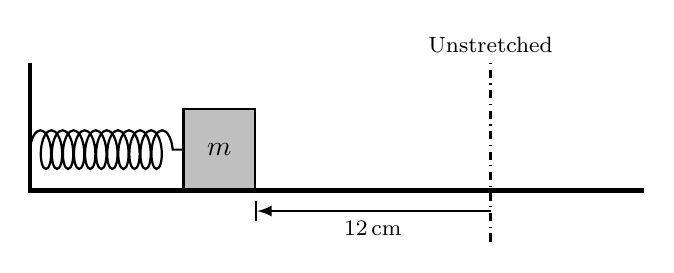
\begin{tikzpicture}[scale=1.3]
      \draw[thick,
        decoration={aspect=.4,segment length=4, amplitude=7, coil},
        decorate] (0,.4)--(1.5,.4);
      \draw[thick,fill=lightgray] (1.5,0) rectangle (2.2,.8) node[midway]{$m$};
      \draw[ultra thick] (0,1.25)--(0,0)--(6,0);
      \draw[|<-,thick] (2.2,-.2)--(4.5,-.2)
      node[midway,below]{\footnotesize\SI{12}{\centi\metre}};
      \draw[dash dot,thick] (4.5,-.5)--(4.5,1.25)
      node[above]{\footnotesize Unstretched};
    \end{tikzpicture}
  \end{center}
  \begin{parts}
    \part[4] What is the speed of the box at the instant the spring is passing
    the point of being compressed by \SI8{\centi\metre}? (It has now moved
    \SI4{\centi\metre} away from the initial compression.)
    
    \uplevel{
      The box reaches maximum speed at equilibrium, when the forces on the box
      are balanced. Note that because of the kinetic friction on the box, the
      equilibrium position is \emph{not} when the spring has fully decompressed.
    }
    
    \part[4] Draw a free-body diagram of the box when it is at equilibrium.

    \part[3] Calulate the spring displacement when the box is at equilibrium
    position.
    
    \part[4] At this equilibrium position, the box's speed is at its maximum.
    What is this maximum speed?

    \uplevel{
      The box loses contact with the spring after the spring has fully
      decompressed. It then slides along the same surface (with $\mu=0.25$)
      until frictional force slows the box to a stop.
    }
    \part[6] How far will the box travel after leaving the spring?
  \end{parts}
  \newpage

  \question In a billiards game, the \SI{170}{\gram} cue ball, travelling
  \SI{.6}{\metre\per\second} forward, hits a stationary \SI{160}{\gram} eight
  ball. After impact, the cue ball rolls away at an angle of \ang{40}
  counter-clockwise from its initial direction, with a speed of
  \SI{.4}{\metre\per\second}.
  \begin{parts}
    \part[7] What is the final \emph{velocity} of the eight ball? (Note that
    the masses of the balls are not the same.)

    \part[5] Find the initial and final kinetic energy of the billiard balls,
    and determine if the collision is elastic or inelastic.
  \end{parts}
  \newpage
  
%  \question[6] A simple pendulum swings freely and rises at the end of
%  its swing to a position 8.5 cm above its lowest point. What
%  is its speed at its lowest point?

%  \question[6] A spring with a spring constant of
%  \SI{450}{\newton\per\metre} hangs vertically from the ceiling of a house. You
%  attach a \SI{2.2}{\kilo\gram} block to it and
%  allow the mass to fall. What is the maximum distance the block will fall
%  before it begins moving upward?

%  \question[10] A car travelling on a flat curved road (no banking)
%  with a radius of \SI{1.e2}{\metre} will skid if the tires do not provide
%  enough traction. Draw a free-body diagram of a \SI{1500}{\kilo\gram} car
%  travelling on the curved
%  road. Calculate the centripetal force required to keep the car travelling at
%  \SI{65}{\kilo\metre\per\hour}. What must the coefficient of friction be
%  between the tires and the ground?

%  \question You and a colleague are on a spacewalk, repairing your
%  spacecraft that has stalled in deep space. Your \SI{69}{\kilo\gram}
%  colleague, initially at rest, asks you to throw her a hammer, which has a
%  mass of \SI{3}{\kilo\gram}. You throw it to her with a forward velocity of
%  \SI{4.5}{\metre\per\second}.
%  \begin{parts}
%    \part[4] What is her velocity after catching the hammer?
%    \part[4] What impulse does the hammer exert on her?
%    \part[4] What percentage of kinetic energy is lost when your colleague
%    caught the hammer?
%  \end{parts}
  
%  \question The Global Positioning System (GPS) uses a ``constellation'' of
%  more than
%  30 satellites to provide accurate positioning for any point on Earth. GPS
%  receivers time radio signals travelling at the speed of light from three of
%  the satellites to find (``triangulate'') the receiver’s position. Signals
%  from one or more satellites provide corrections, eliminating the need for
%  high-accuracy clocks in individual GPS receivers. GPS satellites are in
%  circular orbits at \SI{20000}{\kilo\metre} altitude.
%  \begin{parts}
%    \part[3] What is the approximate orbital period of GPS satellites?
%    \part[3] Item What is the approximate orbital speed of GPS satellites?
%    \part[3] What is the approximate escape speed from the orbital distance?
%    \part[3] The current generation of GPS satellites has a mass of
%    \SI{844}{\kilo\gram}. What is the total energy of such a satellites?
%  \end{parts}

%  \question[6] A \textbf{white dwarf} is a collapsed star with roughly the
%  Sun's mass compressed into the size of Earth. What would be the orbital speed
%  and period for a spaceship in orbit just above the surface of a white dwarf?
  
%  \question A \emph{Schwarzchild singularity} is a theoretical star
%  where the escape velocity from its surface is equal to the speed of light
%  ($v_\text{esc}=c=\SI{2.998e8}{\metre\per\second}$). Such are star will
%  therefore appear completely black, since not even light can escape from it.
%  The radius of a Schwarzchild singularity is called the
%  ``Schwarzchild radius''.
%  \begin{parts}
%    \part[5] Compute the Schwarzchild radius of a star with the same mass as
%      our sun.
%    \part[3] What would be the density of this star?
%  \end{parts}

%  \question[5] A proposed ``space elevator'' can lift a \SI{1000}{\kilo\gram}
%  payload to
%  a height of \SI{150}{\kilo\metre} above Earth's surface. The radius of Earth
%  is \SI{6.37e6}{\metre}, and Earth's mass is \SI{5.97e24}{\kilo\gram}. What
%  is work required to lift the payload to orbit?
  
  \fullwidth{
    \centering
    \textbf{THE FOLLOWING IS A BONUS QUESTION}
  }

  \bonusquestion[10] A \SI{200}{\gram} block ($m$) is released from rest at a
  height of \SI{25}{\centi\metre} on a frictionless \ang{30} incline. It slides
  down the incline and then along a frictionless surface until it collides
  elastically with an \SI{800}{\gram} block ($M$) at rest \SI{1.4}{\metre} from
  the bottom of the incline (see diagram). How much later do the blocks collide
  again? Attach extra work on the next page if more room is needed for your
  calculations.
  \uplevel{
    \centering
    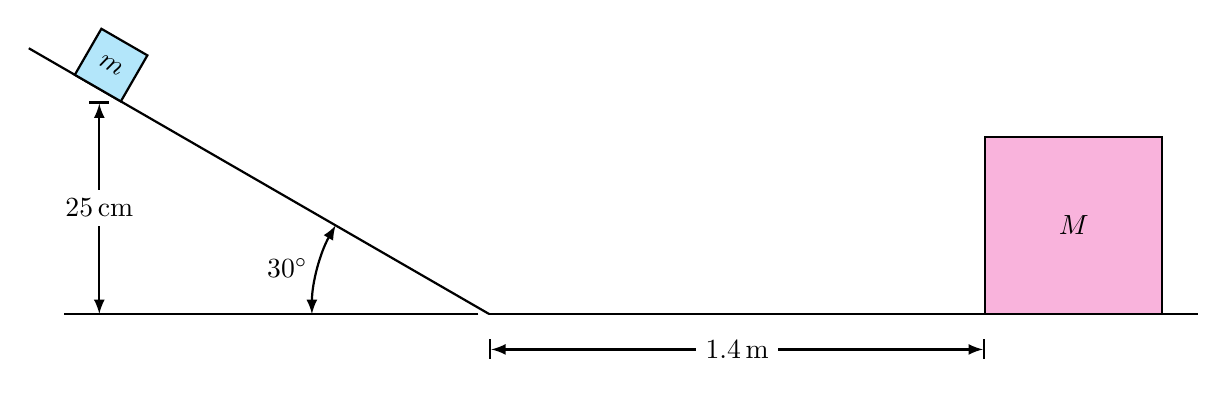
\begin{tikzpicture}[scale=4.5]
      \begin{scope}[thick]
        \draw (0,0)--(2,0);
        \draw[fill=magenta!30](1.4,0) rectangle (1.9,.5) node[midway]{$M$};
        \begin{scope}[rotate=-30]
          \draw (0,0)--(-1.5,0);
          \draw[fill=cyan!30](-1.2,0) rectangle(-1.35,.15)
          node[midway,rotate=-30]{$m$};
        \end{scope}
        \draw (-.03,0)--(-1.2,0);
        \draw[<->](-.5,0) arc(180:150:.5) node[midway,left]{\ang{30}};
        \draw[|<->|](0,-.1)--(1.4,-.1) node[midway,fill=white]{\SI{1.4}\metre};
        \draw[<->|](-1.1,0)--(-1.1,.6)
        node[midway,fill=white]{\SI{25}{\centi\metre}};
      \end{scope}
    \end{tikzpicture}
  }
  
%  \bonusquestion[5] Crooked Olympic commissioners decided to buy and sell
%  gold, hoping to set a new profit record. They conducted all their business in
%  an elevator. They
%  bought and sold at the same price per ounce (an archaic unit of force) which
%  they measured with a vertical spring scale suspended from the ceiling. They
%  always bought their gold when the elevator had a downward acceleration of
%  \SI{2.0}{\metre\per\second\squared} and always sold it when the acceleration
%  was \SI{2.5}{\metre\per\second\squared}
%  upward. Evaluate their percentage profit, based on their buying price.

  
%  \bonusquestion[9] Sadman Whatsizname flees across the flat desert in an
%  armoured vehicle at \SI{72}{\kilo\metre\per\hour} pursued by Storman Norman.
%  He drives off the
%  edge of a cliff \AI{490}{\metre} above a lake of burning oil. Each time he
%  strikes the
%  surface of the lake, he bounces in a peculiar fashion. His horizontal
%  velocity is unchanged, but his vertical velocity instantly reverses direction
%  and decreases in magnitude by exactly \SI{20}{\percent}. What is the maximum
%  width of the lake if Sadman is able to cheat the flames and reach the far
%  shore?
  \end{questions}
\end{document}
